\subsection{Testkonzept Hardware}\label{sec:testkonzeptHardware}
Damit ein reibungsloser Betrieb möglich ist, müssen die einzelnen Hardware Komponenten auf Herz und Nieren geprüft werden. Nachfolgend werden die Testverfahren genauer beschrieben und die Testergebnisse aufgelistet.

\subsubsection*{Schutzmechanismen Batterie}\label{sec:batterie}
Die Batterie weist einige Schutzmechanismen auf, welche alle getestet werden müssen. Als erstes wurde der Tiefentladungsschutz geprüft. Um dies zu testen wurde ein Widerstand der Dimension 9$\Omega$ angeschlossen, was gemäss Berechnung \ref{eq:Entladestrom} einen Entladestrom von rund 411mA zur Folge hatte.

\begin{equation}
\centering
I_{discharge}=\frac{U}{R}=\frac{3.7V}{9\Omega }= 411mA
\label{eq:Entladestrom}
\end{equation}

Während dem Entladevorgang wurde stets die Spannung überwacht, wobei die Spannung von 3.7V auf bis 2.5V absank. Nach dem die 2.5V Schwellenspannung unterschritten wurde, brach der integrierte Batterieschutz die Spannungsversorgung ab. Die Widerstände wurden abgehängt und der gesamte Vorgang wurde kurze Zeit danach mit dem selben Endergebnis wiederholt.
\\
Als nächstes wurde ein Kurzschlusstest durchgeführt, wobei hier der Schwellenstrom gemäss Datenblatt bei 4.8A liegt. Gemäss dem $U=R\cdot I$ Gesetz, wurde ein Widerstand der Grösse von $700m\Omega$ verwendet, um den Grenzwert zu überschreiten. Auch bei diesem Versuch riegelte das PCM den hohen Entladungsstrom ab und schaltete die Versorgungsspannung der Batterie ab.

\subsubsection*{Ladeschaltung der Batterie}\label{sec:batterie}
Für die Ladeschaltung der Batterie wurde wie im Kapitel \ref{sec:Energiespeicher} bereits erwähnt ein Lade-IC verwendet. Dieser reguliert zuerst die Spannung wobei nach Erreichung des Schwellenwertes von $4.2V$ der Strom auf $0A$ herunter reguliert wird. Dieser Vorgang wurde während einem gesamten Ladevorgang der Batterie beobachtet und dokumentiert und ist in Abbildung \ref{fig:LadekurveEmmerich} ersichtlich. Hierbei ist wichtig zu erwähnen, dass dieses Testing nicht die induktive Energieübertragung verwendete, sondern der Fokus auf der Funktionalität des Lade-ICs beschränkt und somit das Netzgerät \glqq Power Supply\grqq\space der Firma \glqq K. Witmer\grqq\space als Spannungsspeisung verwendet wurde. Aus diesem Grund ist auch ein Strom von $400mA$ wie auch eine Ladezeit von lediglich rund $270$ Minuten $(\hat{=} 4.5h)$ ersichtlich was die effektiven Ladewerte mittels induktiver Ladung deutlich unterbietet. Ersichtlich ist nachfolgend die Regulierung der Spannung (blaue Kurve) wie auch die Regulierung des Stromes (rote Kurve).

\begin{figure}[H]
	\begin{center}
		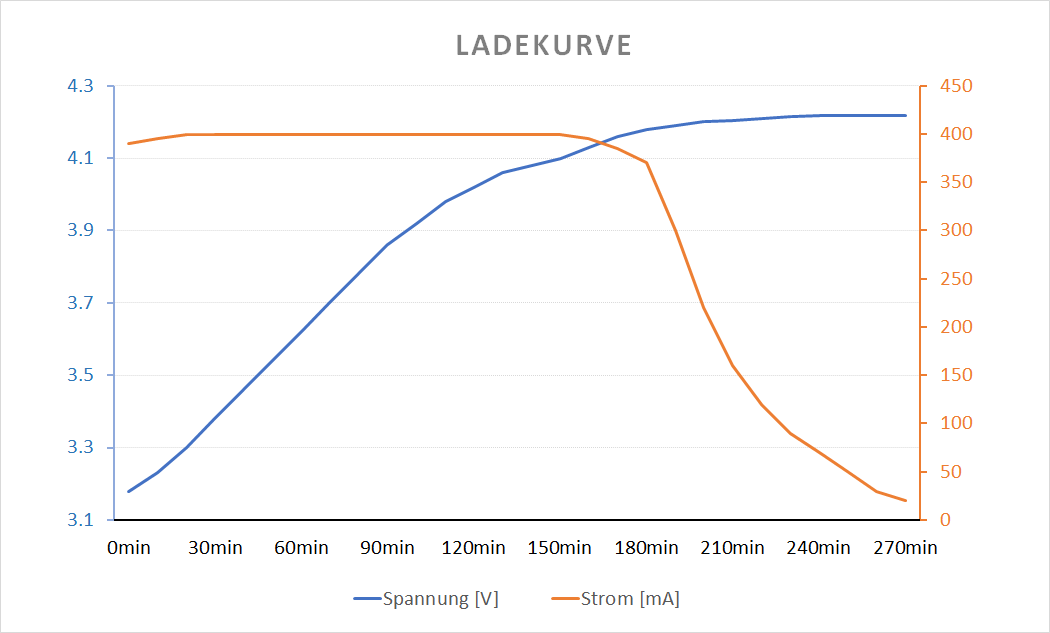
\includegraphics[width=120mm]{data/LadekurveEmmerich.png}
		\caption[Ladekurve Emmerich LI14500]{Ladekurve Emmerich LI14500} %picture caption
		\label{fig:LadekurveEmmerich}
	\end{center}
\end{figure}

Die oben genannten Vorgänge der Spannungs- und Stromregulierung sind in dieser Grafik gut ersichtlich, wobei der Ladevorgang nach dem erreichen von rund 20mA als fertig betrachtet wurde.

\subsubsection*{Induktive Ladeschaltung}\label{sec:batterie}
In diesem Abschnitt werden die Ergebnisse der induktiven Ladeschaltung präsentiert. Nachfolgend zeigt Abbildung \ref{fig:InduzierterStrom} die Abhängigkeit zwischen induziertem Strom und Spannung in Abhängigkeit zur Distanz z zwischen den Induktionsspulen.

\begin{figure}[H]
	\begin{center}
		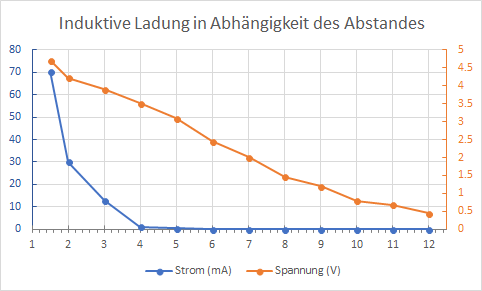
\includegraphics[width=100mm]{data/InduktiveLadung.png}
		\caption[Induzierter Strom in Abhängigkeit der Distanz]{Induzierter Strom in Abhängigkeit der Distanz} %picture caption
		\label{fig:InduzierterStrom}
	\end{center}
\end{figure}

In der Abbildung ist gut sichtbar, dass die Spannung fast linear zur Distanz abnimmt, hingegen der Ladestrom der Batterie extrem schnell klein wird. Aufgrund dieser Erkenntnissen sind wir gezwungen eine möglichst kurze Entfernung zwischen den Spulen einzuhalten weshalb wir eine Ladestation entworfen haben, welche die bestmöglichen Induktionswerte garantiert. Der minimale Abstand welcher beim Ladezyklus erreicht werken kann beträgt rund $1.5mm$. Dieser Abstand entspricht ziemlich genau der Wanddicke des Dōjōs. Bei diesem Abstand resultiert ein an die Batterie gelieferter Strom von maximal $70mA$, wobei die Ladezeit direkt von diesem Strom abhängt. Der Ladezyklus wird in zwei Etappen unterteilt. Bei der ersten Etappe wird die Batterie mit konstantem Strom geladen. Dies hat zur Folge, dass die Spannung von ihrem Minimalwert $3.3V$ auf den Schwellenwert von $4.2V$ reguliert wird. Um auf die notwendige Ladezeit des ersten Ladezyklus zu kommen, kann die Zeit während einer beliebig grossen Spannungsdifferenz gestoppt werden. Generell gilt: Umso grösser die Spannungsdifferenz, desto genauer die Approximation. Die Endzeit der Spannungsregelung kann linear hochgerechnet werden. Da jedoch der Ladezyklus nach vollständiger Spannungsregelung noch nicht abgeschlossen ist, folgt noch die benötigte Zeit für die Stromregelung. Da diese nicht einfach berechnet werden kann, wurde dieser Prozess im Labor durchgeführt und gestoppt. Diese zwei Ladezyklen zusammen gerechnet ergeben die gesamte Ladezeit. Für den Ladezyklus wurden drei unterschiedlich hohe Ströme definiert, welche die Zeit für den Ladezyklus vorgeben. Sie beinhaltet einen schonenden Ladezyklus ($I_{charge}=30mA$), einen normalen Ladezyklus ($I_{2}=50mA$) und einen schnellen Ladezyklus ($I_{3}=70mA$). Die Erreichung dieser drei Ladestufen wird in dieser Arbeit nicht weiter definiert, könnte jedoch durch drei unterschiedliche Spannungsstufen an die Primärspule reguliert werden. Nachfolgend sind die Berechnungen für die jeweiligen Ladezeiten $t_{voltage}$ und $t_{current}$ der drei Stufen, wie auch die gesamte Ladezeit $t_{tot}$ ersichtlich.
\\
\\

\underline{Ladezyklus schonend}
\begin{equation}
\centering
t_{voltage}=\frac{1.1 V}{(\frac{0.006 V}{10 Minuten})}=1'833.3 Minuten= 30h\thickspace 33min
\label{eq:SchonendSpannung}
\end{equation}
\begin{equation}
\centering
t_{current}= 2h\thickspace 7min
\label{eq:SchonendStrom}
\end{equation}

Die gesamte Ladezeit ergibt sich durch Addition der Berechnungen \ref{eq:SchonendSpannung} und \ref{eq:SchonendStrom}.

\begin{equation}
\centering
t_{tot}=t_{slow_{voltage}}+t_{current}=32h\thickspace 27min \sim 32.5h
\label{eq:SchonendGesamt}
\end{equation}
\\
\\


\underline{Ladezyklus normal}
\begin{equation}
\centering
t_{voltage}=\frac{1.1 V}{(\frac{0.0016 V}{10 Minuten})}=687.5 Minuten= 11h\thickspace 28min
\label{eq:NormalSpannung}
\end{equation}
\begin{equation}
\centering
t_{current}= 46min
\label{eq:NormalStrom}
\end{equation}

Die gesamte Ladezeit des normalen Ladezyklus ist nachfolgend in \ref{eq:NormalGesamt} ersichtlich.

\begin{equation}
\centering
t_{tot}=t_{voltage}+t_{current}=12h\space 46min \sim 13h
\label{eq:NormalGesamt}
\end{equation}
\\
\\


\underline{Ladezyklus schnell}
\begin{equation}
\centering
t_{voltage}=\frac{1.1 V}{(\frac{0.0265 V}{10 Minuten})}=415.1 Minuten= 6h\thickspace 55min
\label{eq:SchnellSpannung}
\end{equation}
\begin{equation}
\centering
t_{current}= 1h\thickspace 18min
\label{eq:SchnellStrom}
\end{equation}
Die gesamte Ladezeit gemäss Berechnung \ref{eq:SchnellGesamt} ergibt sich durch Addition der Berechnungen \ref{eq:SchnellSpannung} und \ref{eq:SchnellStrom}.

\begin{equation}
\centering
t_{tot}=t_{voltage}+t_{current}=7h\thickspace 41min \sim 8h
\label{eq:SchnellGesamt}
\end{equation}
\\
\\
 
Augenfällig ist die kurze Ladezeit von lediglich rund $8$ Stunden beim schnellen Ladezyklus (Berechnung \ref{eq:SchnellGesamt}). Da sich jedoch bei einem Strom von $70mA$ die Spule mehr erwärmt als beim Ladezyklus mit $50mA$, wird vorgeschlagen, dass bei genügend Zeit der normale Zyklus mit $50mA$ gestartet wird. Dieser ist zwar um rund $5$ Stunden langsamer, jedoch nachhaltiger für die eingebauten Materialien.


\subsubsection*{Inbetriebnahme der induktiven Ladeschaltung}\label{sec:erkenntnisse}

Der erste Prototyp der Pulsschaltung für die Induktion wurde mithilfe eines NE555 realisiert. Dabei wurden als Widerstände Potentiometer eingebaut, mit welchen die Resonanzfrequenz des LC-Gliedes gesucht werden sollte.

Der allererste Versuch ergab eine Übertragung von 5mA bei einer Taktfrequenz von 10kHz. Es stellte sich relativ schnell heraus, dass die Taktfrequenz viel zu tief war. Das konnte durch die Veränderung der Taktfrequenz der Pulsschaltung festgestellt werden. Bei höherer Taktfrequenz wurde die Übertragung besser.

Da die Taktfrequenz der NE555-Prototypenschaltung aufgrund der Wahl des Potentiometers auf $10kHz$ begrenzt war, wurde nun in weiteren Schritten mit dem Frequenzgenerator der $2n3055$ Leistungstransistor angesteuert. Des Weiteren wurde das C aus dem LC-Glied ausgebaut, um so das spezifische Maximum der Spule zu finden.

So wurde nun mit konstanter Eingangsspannung und variabler Taktfrequenz die Spule getestet. Mit höher werdender Frequenz wurde die Übertragung besser. Um diese noch weiter zu verbessern empfiehlt sich bei der Taktfrequenz einen Duty Cycle von möglichst $50\%$ zu erzielen.

Es erwies sich, dass bei der Taktfrequenz von $93kHz$ die beste Übertragung zustande kam. Bei höheren Frequenzen war diese wieder rückläufig. Da nun die optimale Frequenz gefunden und die Induktivität der Spule bekannt war ($14.9\mu H$), konnte der ideale Kopplungskondensator berechnet werden. Dies ergab, unter Berücksichtigung der E-Reihen, einen $220nF$ Kondensator als ideal. Damit die Spule nicht zu heiss werden und der Isolierlack nicht zu schmelzen beginnt, wurde der Strombegrenzungswiderstand des $2n2222$ mit $2\Omega$ definiert. Die Berechnung hierzu ist im oberen Text zu finden. Somit sind alle benötigten Bauteile bekannt.

\begin{figure}[H]
	\begin{center}
		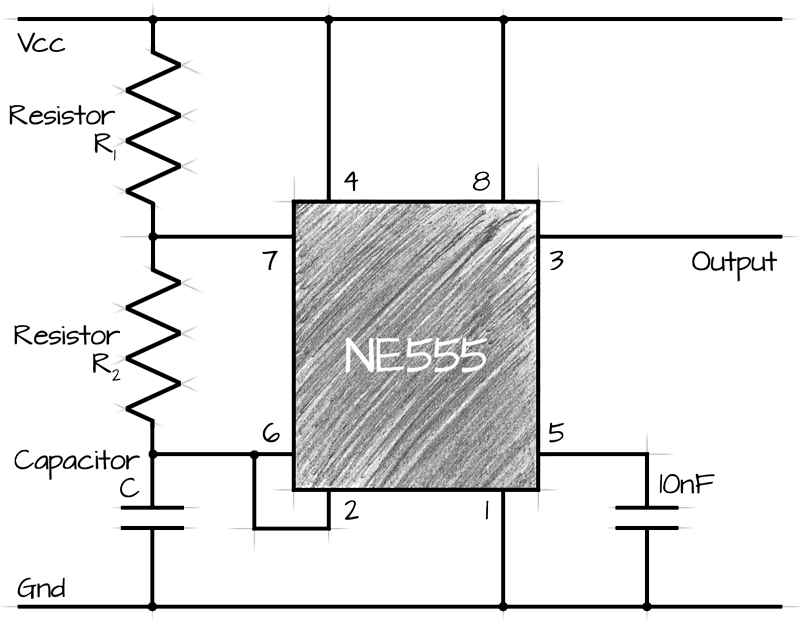
\includegraphics[width=80mm]{data/Ne555circuit.png}
		\caption[Verwendete Timerschaltung NE555 als Pulsquelle]{Verwendete Timerschaltung NE555 als Pulsquelle} %picture caption
		\label{fig:NE555}
	\end{center}
\end{figure}

$C = 1nF$\\
$R_{1} = 200\Omega$\\
$R_{2} = 9 k\Omega$\\

Mit diesen Werten konnte nach dem Gleichrichter, bei einer Übertragungsdistanz von einer Standard-Platinen dicke, eine Leerlaufspannung von ca. $17V$ und ein Kurzschlussstrom ca. 300mA gemessen werden. Es gilt jedoch zu beachten, dass diese Werte ohne Last gemessen wurden. 

Da nun die Induktionsstufe funktioniert wird diese nun um die Ladeschaltung erweitert. Hier ergab sich folgendes Problem:

Die Eingangsspannung des Lade-IC’s darf nicht mehr als $6.5$ Volt betragen. Da die Receiverspule sich im inneren des Dōjōs befindet und dadurch nur eine sehr geringe Baugrösse besitzen darf, kann diese zwangsläufig keine grossen Leistungen erbringen. Dies bedeutet, dass akzeptabel Ladeströme nur mit genügend hohen Spannungen erzeugt werden können.

Um dies zu erzielen wurde versucht, einen Spannungsregler einzubauen, um den übertragenen Strom bei zuhalten, jedoch die Spannung zu begrenzen. Das Ergebnis davon war jedoch ziemlich bescheiden. Der so entstehende Energieverlust ist ziemlich gross und ausserdem kam es vereinzelt vor, dass der Lade-IC trotzdem kaputt ging, da der Spannungsregler nicht sauber regelte. 

Die Ideale Lösung wäre natürlich einen geeigneteren Lade-IC zu nehmen. Da jedoch die Validierung desjenigen bereits durchgeführt wurde und nicht genügend Zeit vorhanden war diesen erneut zu bestellen wurde sich entschieden die Transceiver Schaltung ein wenig anzupassen.

Dabei gibt es folgende Möglichkeiten. Man kann die Eingangsspannung absenken. Dies beeinflusst jedoch auch den Übertragenen Strom exponentiell, da einerseits eingangsseitig mit weniger Spannung auch weniger Strom durch die Spule fliess und andererseits auch der Leistungsstransistor nicht sauber durchgesteuert wird da dieser ebenfalls an der gleichen Versorgungsspannung hängt und somit sein Pulssignal beeinflusst. Die zweite Möglichkeit ist die Taktfrequenz verringern. Dadurch wird die Induzierte Spannung ebenfalls abgesengt was ebenfalls den Strom exponentiell beeinflusst. Die dritte Möglichkeit wäre die Übertragungsdistanz zu verringern. Da aber sichergestellt werden wollte, dass der Dōjō-Boden dennoch eine gewisse Stabilität aufweisen sollte wurde diese Distanz der Platinendicke beigehalten.

Somit wurde die Schaltung lange ausgetestet um die beste Kombination zu erzielen. Das beste Resultat ergab die Kombination zwischen einer Taktfrequenz von ca 80kHz und einer Eingangs Spannung von $8.3V$. Dies lässt sich damit erklären das leichtes Absenken der beiden Möglichkeiten den Strom nicht so stark beeinflusst. Des Weiteren wurde der Strombegrenzungswiderstand auf $1.5\Omega$ verringert da sich die Eingangs Spannung verringert hat und ausserdem der Stromfluss durch die Spule damit erhöht wurde. 

Diese Anpassungen fielen ebenfalls zu Gunsten des Energiemanagements, jedoch ist dies eine stabile Variante für die ersten Prototypen. Durch die Anpassungen wird die überschüssige Energie in Form von Wärme an dem Transceiver Spule abgegeben. Die Test ergaben, dass so die Batterie bei einer Spannung von 4.7V mit 70mA geladen wird. Es ist ebenfalls möglich kurzzeitig mit einem höheren Strom zu laden, wenn die Eingangs Spannung nur geringfügig erhöht wird. (bis zu 120mA). Jedoch ist die Hitzeentwicklung hierbei so gross, dass nach einer gewissen Zeit die Übertragung zusammenbricht. Deshalb ist zu empfehlen die angegebenen Werte nicht zu überschreiten um eine dauernde Funktionalität zu gewährleisten.

Die Werte der oben beschriebenen angepassten Pulsschaltung sind folgende:\\
C: 1nF\\
R1: 200 $\Omega$\\
R2:9 k$\Omega$\\


\subsubsection*{LC-Filter} \label{sec:Validierung LC-Filter}
Die Validierung des LC-Filters wurde mittels eines $500Hz$ Sinus Signals erledigt. Dabei wurde sowohl ohne Filter wie auch mit Filter eine KO Bild aufgenommen. Abbildung \ref{fig 500Hz ohne Filter} zeigt das Signal ohne Filter. Rot angezeigt ist die FFT des Signals. In Abbildung \ref{fig 500Hz mit Filter} ist das Signal und die FFT davon mit dem LC-Filter. 


\begin{figure}[H]
	\begin{center}
		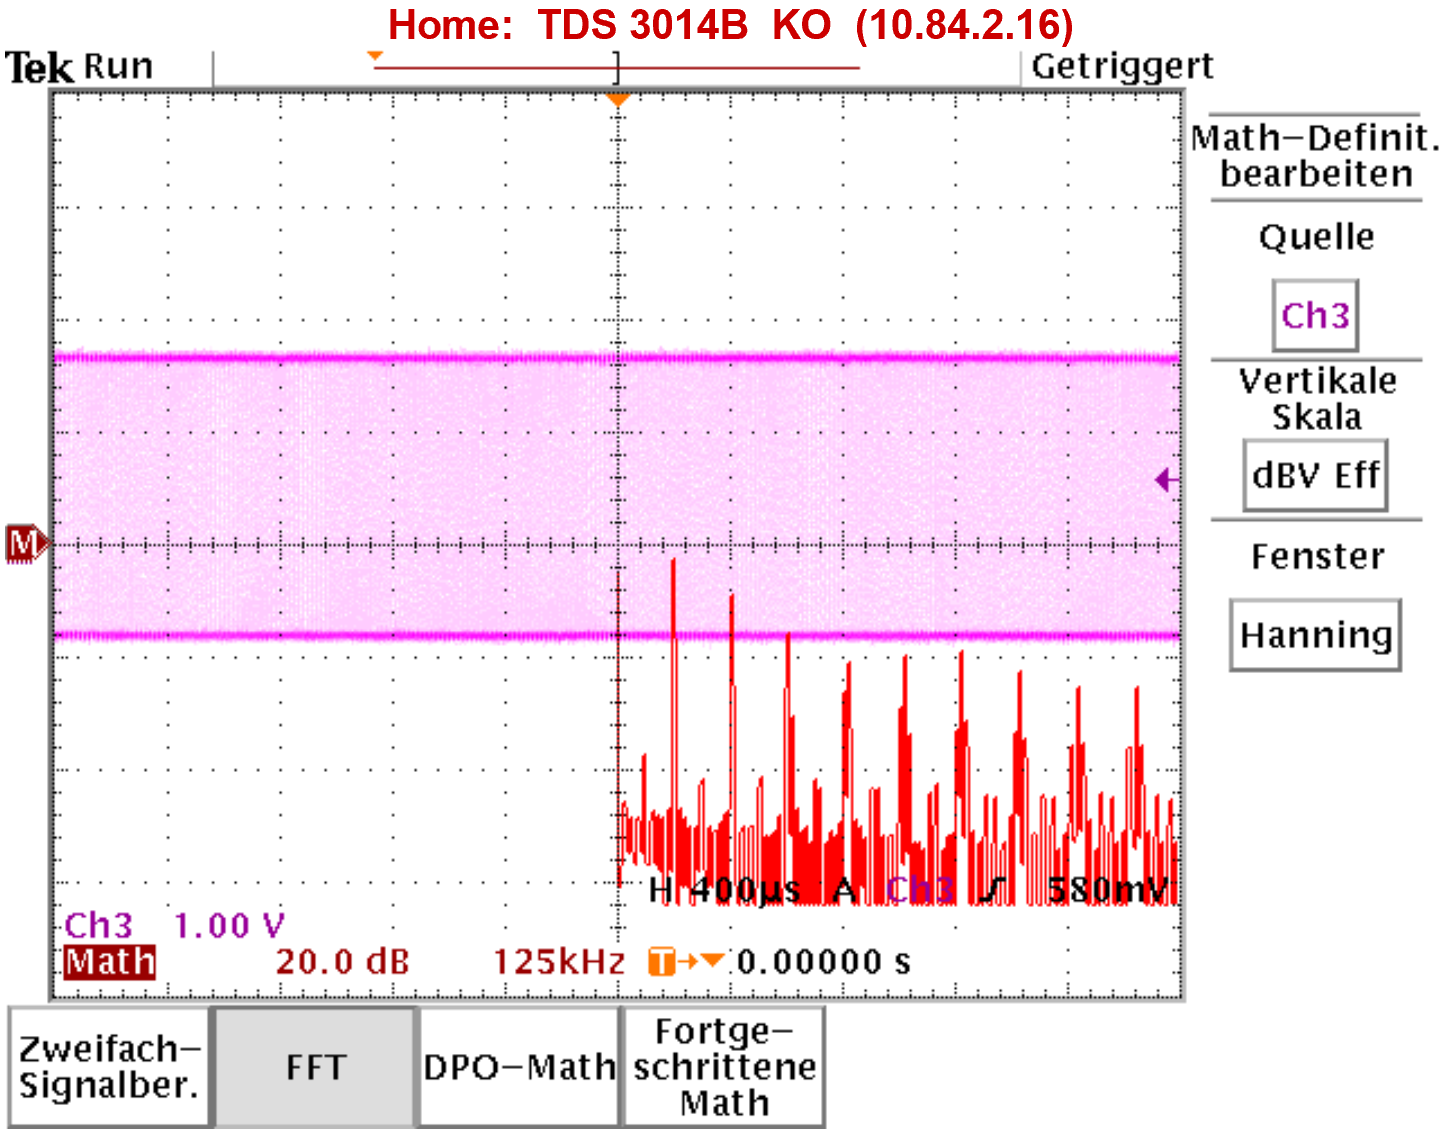
\includegraphics[width=120mm]{data/500Hz_Sin_ohne_Filter_FFT.png}
		\caption[500Hz Sinus Signal und FFT ohne LC-Filter]{500Hz Sinus Signal und FFT ohne LC-Filter} %picture caption
		\label{fig:500Hz ohne Filter}
	\end{center}
\end{figure}

\begin{figure}[H]
	\begin{center}
		\includegraphics[width=120mm]{data/500Hz_Sin_mit_Filter_FFT.png}
		\caption[500Hz Sinus Signal und FFT mit LC-Filter]{500Hz Sinus Signal und FFT mit LC-Filter} %picture caption
		\label{fig:500Hz mit Filter}
	\end{center}
\end{figure}

Durch die beiden KO Aufnahmen wurde ersichtlich, dass durch den Filter ein deutlich besseres und weniger verrauschtes Signal rekonstruiert wird. Somit ist der LC-Filter notwendig, da mit ihm die Schaltfrequenzen des PWM Ausgangs unterdrückt werden.
